
\documentclass[12pt,letterpaper]{article}
\usepackage{../pset_2024}


\qa{q} % a="answers only"; q ="questions only"; b="both"
\usepackage{../qa}

%figuring out points per question: quiz component currently at 28 points
%so need 72 points for part II, over eight subquestions. so avg 9 points per subquestion 

%other question ideas: have them discuss whether they think the control hypothesis is correct or not. 


\begin{document}


\psintro{Problem Set 4: Time Travel}

\newpage

%\fbox{\parbox{150mm}{\emph{Warning:} At this point, you're doing philosophy. Keep in mind that even if a problem is murky, it can be addressed in more or less thoughtful ways: a good answer will reveal that you've understood the complexity of the underlying terrain and that you've given the issue serious thought.}



\subsection*{Part I (Quiz on Canvas: 30 points)} 



\begin{enumerate}


\item \question{Recall that for a time-travel story to be consistent, it must never give us conflicting descriptions of a single point in the narrative's timeline.

With that in mind, determine whether each of the the following stories can be interpreted as a consistent time travel story. (Make sure you interpret them as stories about ordinary time, rather than super-time, and that you interpret them as time travel stories rather than world-travel stories.)}

\begin{enumerate}






\item \question{After doing badly in an exam, you resolve to travel back in time to give yourself a hint before the exam takes place. You successfully travel back in time but mistakenly hand your earlier self the wrong hint and end up doing even worse on the exam. (2~points)}




\item \question{In your youth, you discover plans to build a time-machine under your bed. You successfully build a time machine, only to discover that time travel isn't really to your liking. The past is much too dangerous and the future much too warm. So you decide to destroy your time machine. Just to be on the safe side, you use it one last time to travel back in time, and you destroy the plans that are lying under your bed, before your younger self has a chance to look at them. (2~points)}



\item \question{As a child, Oscar goes for a walk in the forest. For a few seconds, he experiences the odd sensation of being watched. Many years later, he uses a time machine to travel back to that fateful day. He finds a good hiding place in the forest and spends a few seconds watching his younger self. As an old man, he again uses a time machine to travel back to that fateful day. He finds an even better hiding place and---like a champion creep---spends a few seconds watching his middle-aged self watch his younger self. (2~points)}


\item \question{A team of lepidopterists travels back in time to the Paleogene, hoping to catch a glimpse of early butterflies. The team is cautioned not to interfere with the past in any way. But accidents happen. As they are completing their journey, one of the scientists steps on a branch and startles a butterfly. When the team returns to the present, they are confronted with changed world. Land octopuses have conquered the Earth and rule with an iron tentacle. A small interference in the past has made a big difference to the future. (2 points)}


\item \question{At time $t$ you wake up to find plans for building a time machine in your desk drawer. You use the plans to build a time machine, and spend many happy years traveling through time. During one of your travels you go back to time $t$ and leave the plans in your younger self's desk drawer. (2 points)}



\end{enumerate}

\item[2.--7.] See \textbf{additional four questions} (\#2--\#5) on Canvas Quiz for Part I (20 points)!



\end{enumerate}



%%%%%%
%PART II
%%%%%%
%\newpage
\subsection*{Part II (Submit PDF on Canvas: 70 points)} 
\begin{enumerate}
\setcounter{enumi}{7}





\item \question{Recall the Control Hypothesis:

\begin{description}
\item[Control Hypothesis]
An agent acts freely in doing $X$ if and only if: (1) she does $X$ by making a certain decision, and (2) she is in a position to do something other than $X$ by making a different decision.
\end{description}
Now consider the following scenarios:}



\begin{enumerate}

\item \question{\begin{quote}Felix is on his way to the bookstore to buy a book. You know him well enough to know that he only likes to read detective stories. So you know from the start that he will choose a detective story. And sure enough: he leaves the bookstore with a detective story, even though he was in a position to choose any book he wanted.
\end{quote}

According to the Control Hypothesis, did Felix act freely in choosing a detective story? Keep in mind that you were able to predict that he would pick a detective story from the start. (5 points; don't forget to justify your answer)}


\vspace{3mm}
\item \question{\begin{quote}Bruno is on his way to kill Grandfather. You know that Grandfather is Bruno's grandfather.\footnote{Also, you know that there is no funny business: no rising up from the dead, no frozen sperm, no replicated DNA, etc.} So you know from the start that Bruno will fail. And sure enough: Bruno has a change of heart at the last minute and decides to put down the gun, even though he was in a position to make a different decision and pull the trigger instead.
\end{quote}
According to the Control Hypothesis, did Bruno act freely in putting down his gun? Keep in mind that you were able to predict that he wouldn't kill Grandfather from the start. (5 points; don't forget to justify your answer)}


\vspace{3mm}
\item

\question{
	\begin{quote}
After an hour of good fun, you decide to leave the party early and spend the rest of the evening at home. Unbeknownst to you, your hosts were finding you a bit tedious, so they were about to ask you to leave just as you left. So, had you instead decided to stay a little longer, you wouldn't have been able to: you would have been forced to leave early anyway. 
\end{quote}
According to the Control Hypothesis, did you act freely in leaving the party early? Is that answer intuitively correct?} (10 points)


\end{enumerate}

%\newpage

%\com{
\item 
  \question{
    Describe how you could use a time machine to give yourself an extension on this problem-set in a consistent manner.
    Assume that you get the time machine on Sunday 03/31/24 and that the problem set is due on Sunday 04/07/24.
    (10 points)
  }
% (Alternatively, if you think it's not possible to give yourself an extension, explain why not)
%As far as you know, you have never interacted with yourself in the past, and no one has any reports of you in the past. 


%}


\newpage


\item \question{
  % Very roughly, to \textit{causally explain} (or `mechanistically explain') how event $x$ occurs (or why it occurs) is to describe a (continuous) sequence of causes and effects leading to $x$'s occurrence, where causes strictly precede their effects in time (assume causation is temporally asymmetric). 
  Consider the following scenario:
}

\begin{enumerate}
%\com{ %left out in 2022 version 
\item[] \question{\begin{quote}On your 21st birthday, an elderly stranger hands you a nautically themed clock. The clock is strikingly beautiful---mesmerizing even, with its moving boats and cuttlefish. Many years later, in your old age, you travel back in time to your 21st birthday and hand the clock to your younger self.
\end{quote}

\vspace{1.5mm}

In this scenario, is there a {causal explanation} to be given about how the clock was originally built? If so, spell it out. If not, explain why not. (10 points)
}


\vspace{3mm}
%}

\com{ %left out in 2023 version 
\item \question{\begin{quote}Olivia travels to the past in an effort to kill her grandfather before he has any children. On pain of contradiction, Olivia will fail to kill Grandfather.\footnote{As usual, we are assuming no funny business: no rising up from
the dead, no frozen sperm, no replicated DNA, etc.}\end{quote}

Extend the story so that it entails a causal explanation of why Olivia fails to kill Grandfather. (10 points)}

}




\end{enumerate}


\item \question{Consider the following scenario:

\begin{quote}You're wondering whether to study for tomorrow's biology exam. It's a hard exam and you won't pass unless you study. Just then you see your good friend Amy emerge from a time machine. She announces that she's been to the future and has seen you pass the exam. Amy is totally reliable, so you can be 100\% confident that you will pass the exam. 
\end{quote}
Does this scenario entail that you'll pass even if you don't study? (10 points; don't forget to justify your answer.)}


%(A ``yes'' answer could in principle get credit, if it's sufficiently justified.)}


\com{
\item \question{On April 2, 2023, Bruno enters a time machine to travel to December 31st, 1999. In eager anticipation of his journey, Bruno says ``Soon I will witness the turn of the millennium.'' Use the distinction between personal time and external time to explain how Bruno's statement can be interpreted as a consistent statement. (3 points)}
} %end com 

\com{
\item \question{The course materials describe a toy model of time travel. The diagram below depicts a wormhole within the world of the toy model. The points represented by \emph{W-} are identified with the points represented by \emph{W+}. Particle $A$ jumps to the future when its spacetime trajectory reaches the wormhole from outside the wormhole region; particle $B$ jumps to the past when its spacetime trajectory reaches the wormhole from inside the wormhole region.


\begin{center}
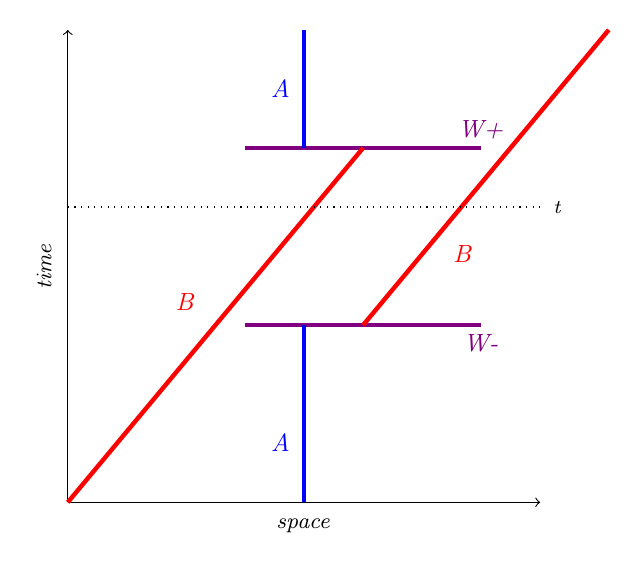
\begin{tikzpicture}[scale = 0.75]
\draw[->] (0,0) -- (0,8); % time axis
\draw[->] (0,0) -- (8,0); % space axis
\node at (4,-0.4) {\footnotesize \emph{space}}; % space label
\node at (-0.4,4) {\footnotesize \rotatebox{90}{\emph{time}}}; % time label

\draw[ultra thick, violet] (3,6) -- (7,6); % Line W+
\node[violet] at (7,6.3) {\small \emph{W+}}; % W+'s label
\draw[ultra thick, violet] (3,3) -- (7,3); % Line W-
\node[violet] at (7,2.7) {\small \emph{W-}}; % W-'s label

\draw[ultra thick, blue] (4,0) -- (4,3); % A's timeline, part 1
\node[blue] at (3.6,1) {\small \emph{A}}; % A's label, part 1
\draw[ultra thick, blue] (4,6) -- (4,8); % A's timeline, part 2
\node[blue] at (3.6,7) {\small \emph{A}}; % A's label, part 2
%\node at (4,3.3) {\footnotesize $p$}; % p label
%\node at (4,5.7) {\footnotesize $p$}; % p label


\draw[ultra thick, red] (0,0) -- (5,6); % B's timeline, part 1
\node[red] at (2,3.4) {\small \emph{B}}; % B's label, part 1
\draw[ultra thick, red] (5,3) -- (9.16,8); % B's timeline, part 2
\node[red] at (6.7,4.2) {\small \emph{B}}; % B's label, part 2
%\node at (6,6.4) {\footnotesize $p'$}; % p label
%\node at (6,2.6) {\footnotesize $p'$}; % p label

\draw[dotted] (0,5) -- (8,5); % time t line
\node[black] at (8.3,5) {\scriptsize \emph{t}}; % time t label

%\draw[dotted] (0,1.7) -- (8,1.7); % time t line
%\node[black] at (8.3,1.7) {\scriptsize \emph{t}}; % time t label
%
%\draw[dotted] (0,5.2) -- (8,5.2); % time t line
%\node[black] at (8.3,5.2) {\scriptsize \emph{t$'$}}; % time t label


\end{tikzpicture}
\end{center}
Note that only one particle---particle $B$---exists at time $t$, though $B$ experiences time $t$ twice. 

Now consider a different diagram:

\begin{center}
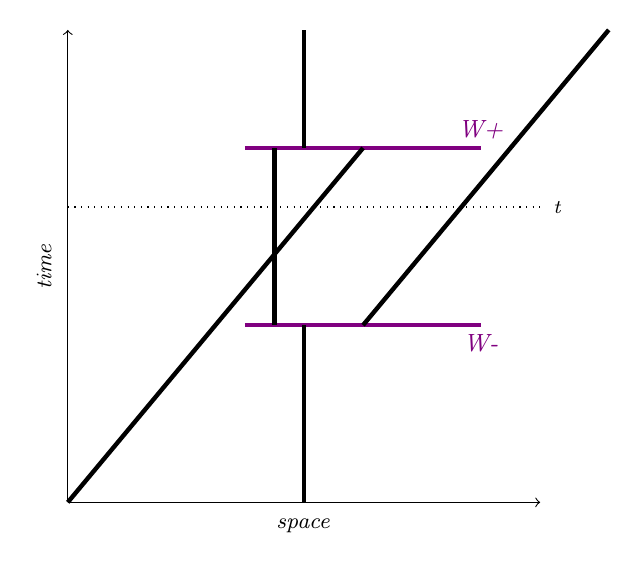
\begin{tikzpicture}[scale = 0.75]
\draw[->] (0,0) -- (0,8); % time axis
\draw[->] (0,0) -- (8,0); % space axis
\node at (4,-0.4) {\footnotesize \emph{space}}; % space label
\node at (-0.4,4) {\footnotesize \rotatebox{90}{\emph{time}}}; % time label

\draw[ultra thick, violet] (3,6) -- (7,6); % Line W+
\node[violet] at (7,6.3) {\small \emph{W+}}; % W+'s label
\draw[ultra thick, violet] (3,3) -- (7,3); % Line W-
\node[violet] at (7,2.7) {\small \emph{W-}}; % W-'s label

\draw[ultra thick] (4,0) -- (4,3); % A's timeline, part 1
%\node[blue] at (3.6,1) {\small \emph{A}}; % A's label, part 1
\draw[ultra thick] (4,6) -- (4,8); % A's timeline, part 2
%\node[blue] at (3.6,7) {\small \emph{A}}; % A's label, part 2


\draw[ultra thick] (0,0) -- (5,6); % B's timeline, part 1
%\node[red] at (2,3.4) {\small \emph{B}}; % B's label, part 1
\draw[ultra thick] (5,3) -- (9.16,8); % B's timeline, part 2
%\node[red] at (6.7,4.2) {\small \emph{B}}; % B's label, part 2

\draw[ultra thick] (3.5,3) -- (3.5,6); % C's timeline

\draw[dotted] (0,5) -- (8,5); % time t line
\node[black] at (8.3,5) {\scriptsize \emph{t}}; % time t label


\end{tikzpicture}
\end{center}
Assuming the laws of the toy model are in place, how many different particles exist at time $t$? (8~points; don't forget to explain your answer)
}

} %end com 


\item \question{There is a famous scene in the film \emph{The Matrix} in which the Oracle predicts that Neo will break a vase. (You can find it online by searching ``matrix oracle vase".\footnote{Or you can go here: \url{https://www.youtube.com/watch?v=eVF4kebiks4}}) }

\begin{enumerate}
\item \label{neo-a}
\question{Describe a consistent time travel story that uses time travel to explain how the Oracle acquires the information necessary to issue her successful prediction. \\ (10 points)}


\item \question{Neo breaks the vase after turning partially around. Does the Control Hypothesis entail that, according to the story you gave in your response to (\ref{neo-a}), Neo fails to act freely in turning around? (10 points)}


\end{enumerate}


%left out for variety in 2022-23
\com{
\item \question{Bruno travels back in time to kill his grandfather, to a time before his grandfather
had any children. Will he succeed? (Assume no funny business: no rising up from
the dead, no frozen sperm, no replicated DNA, etc.) (20 points)

\begin{itemize}
\item If you think the answer is ``yes'', tell a consistent story that makes clear how it is that Bruno succeeds.

\item If you think the answer is ``no", tell a consistent story that makes clear why Bruno does not succeed.


\end{itemize}
}


}





\end{enumerate}

\end{document}


\question{
\subsection*{Optional:}

Is contemporary physics compatible with time travel? Alan Guth, who is a famous physicist at MIT, tackled this question during a visit to \emph{Paradox and Infinity}, a few years ago. You can check out his lecture here: 
\begin{center}
  \includegraphics[width=2.9cm]{guthqrcode.png}\\
\url{bit.ly/2ToPthV}
\end{center}


}





